
\begin{frame}{Motivation : Maillage hexaédrique}
    \centering
    
    \begin{minipage}[c]{0.48\textwidth}
    \centering 
    \textbf{Orthogonal fields}\\
    \vspace{0.3cm}
    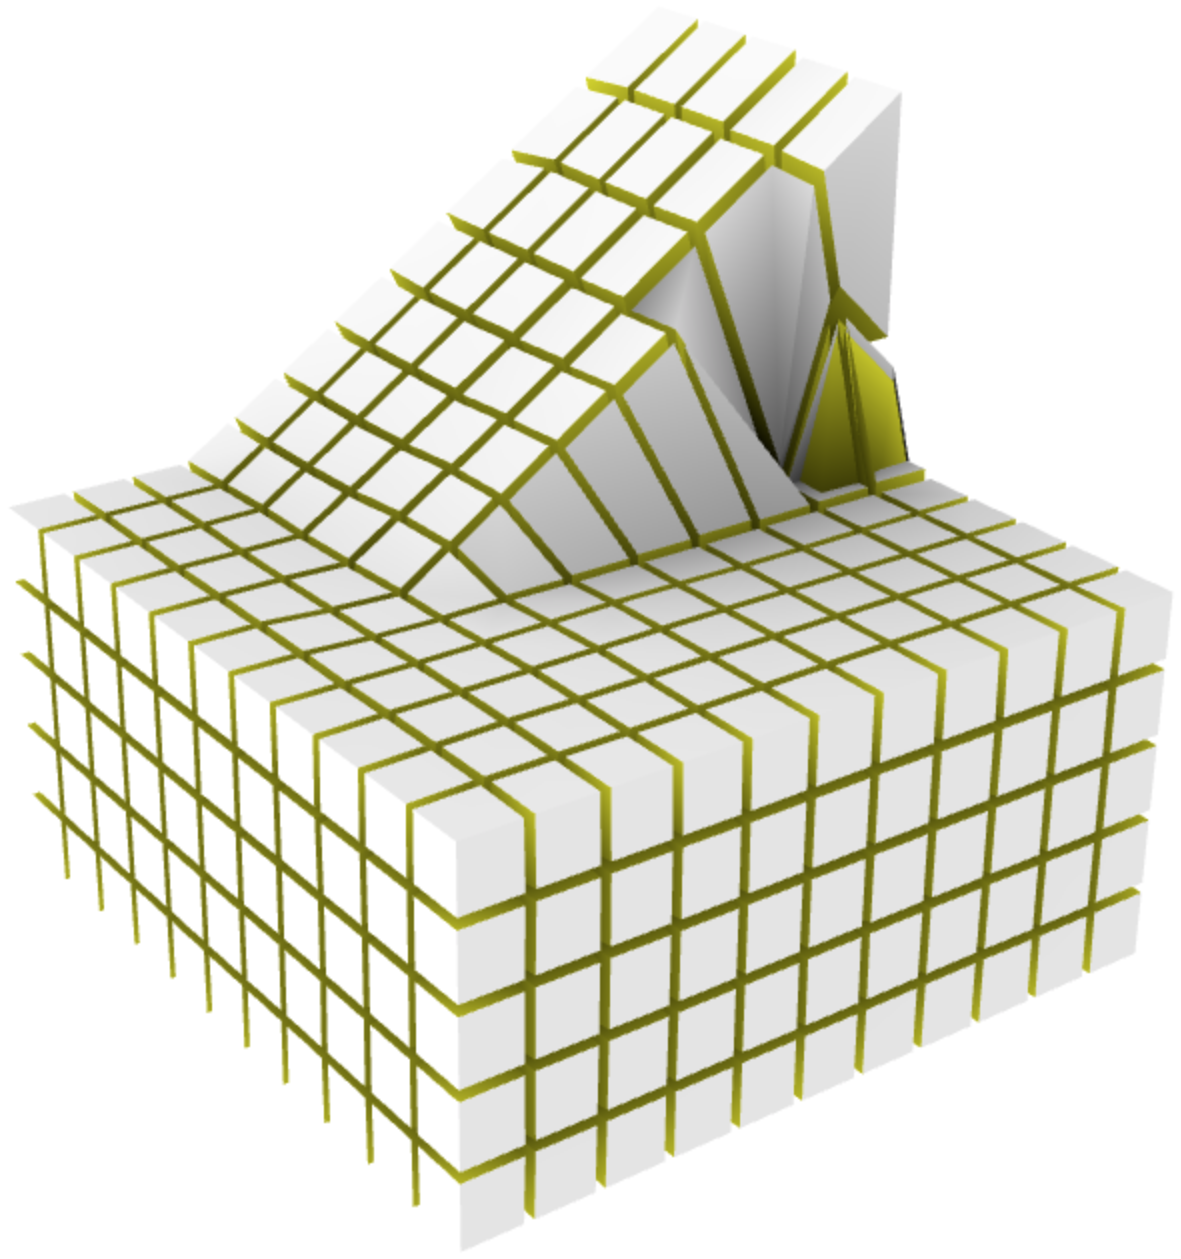
\includegraphics[width=.7\linewidth]{img_spm_ff/slope_ortho_front.png}
    \end{minipage}%
    \hfill\vline\hfill
    \begin{minipage}[c]{0.48\textwidth}
    \centering 
    \textbf{Non-orthogonal fields}\\
    \vspace{0.3cm}
    
\includegraphics[width=.7\linewidth]{img_spm_ff/slope_northo_front.png}
    \end{minipage}
    
    \vspace*{0.3cm}
    \begin{itemize}
        \item Ce travail propose une représentation polynomiale des repères.
        \item Cette représentation permet l'optimisation de champ de repère 3D non-orthogonaux.
    \end{itemize}
    
\end{frame}

\begin{frame}{Polynôme représentant un repère à 3 directions}
    \centering
    \small
    $\mathcal{U} = \left\{\vec{u},\ -\vec{u},\ \vec{v},\ -\vec{v},\ \vec{w},\ -\vec{w}\right\}$ est représenté par un polynôme \\
    \textbf{restreint à la sphère unité}
    %$$P_\mathcal{U} \colon s \mapsto \langle \vec{u},\ s\rangle^{4} +  \langle \vec{v},\ s\rangle^{4} +  \langle \vec{w},\ s\rangle^{4}$$
    $$ P_\mathcal{U}(\vec{s}) = \langle \vec{u},\ \vec{s}\rangle^{4} +  \langle \vec{v},\ \vec{s}\rangle^{4} +  \langle \vec{w},\ \vec{s}\rangle^{4}, \ \ \   \forall \vec{s} \in {\rm I\!R}^3, \lVert \vec{s} \rVert = 1$$
    
    \vspace*{.5\baselineskip}
    \includegraphics[width=0.33\linewidth]{img_spm_ff/sperical_3dir4.png}
    \ \ \ \ \ \ \ \ \ \ \ 
    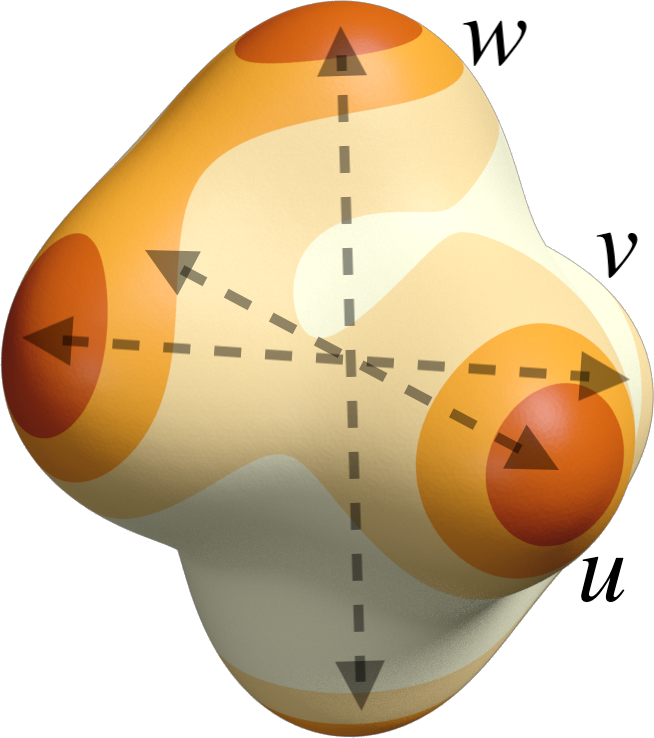
\includegraphics[width=0.3\linewidth]{img_spm_ff/sperical_3dir4_rot.png}
    %\begin{align*}
     %  p_c \colon & s \mapsto \langle u,\ s\rangle^{4} +  \langle v,\ s\rangle^{4} +  \langle w,\ s\rangle^{4} \\
     %  & \mathcal{S}_{\{0, 1\}}^3 \to {\rm I\!R}
    %\end{align*}
\end{frame} 
\begin{frame}{Spherical Harmonic basis}
    \centering
    \begin{overprint}
    \onslide<2> \centering
    Avec un repère orthogonal, nous retrouvons les résultats antérieurs\\
    
    %Polynomials of 3D orthogonal frames can be decomposed as:
    \begin{minipage}[c]{0.24\textwidth}
        \centering
          \vspace*{.5\baselineskip}
          \hfill
        \includegraphics[width=0.6\linewidth]{img_spm_ff/sperical_3dir4.png}
    \end{minipage}
    \begin{minipage}[c]{0.74\textwidth}
        %\centering
        %\includegraphics[width=0.33\linewidth]{sperical_3dir4.png}
        $$P_\mathcal{U}(s) = const \cdot Y_{0, 0} + \sum_{m = -4}^4{{\color{green}c_{4, m}(\mathcal{U})}Y_{4,m}(s)}$$ 
    \end{minipage}
    
    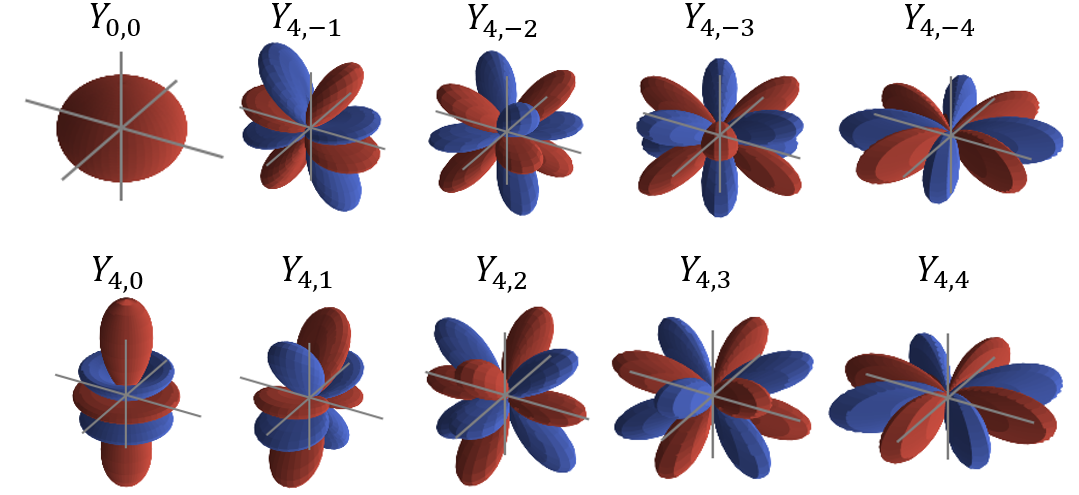
\includegraphics[width=.8\linewidth]{img_spm_ff/ortho_harmonic_decompo.PNG} 
    
    \onslide<1> \centering
        La décomposition de $P_\mathcal{U}$ dans la base des harmoniques sphériques simplifie $dist(\mathcal{U}_i, \mathcal{U}_j)$ \\
    
     %$2^{nd}$ order terms are necessary for non-orthogonality:
    %$$P_\mathcal{U}(s) = const \cdot Y_{0, 0} + \sum_{\ell \in \{2, 4\}} \sum_{m = -\ell}^\ell{{\color{green}c_{\ell, m}(\mathcal{U})}Y_{\ell,m}(s)}$$ 
    
    \begin{minipage}[c]{0.19\textwidth}
        \centering
          \vspace*{.5\baselineskip}
          \hfill
        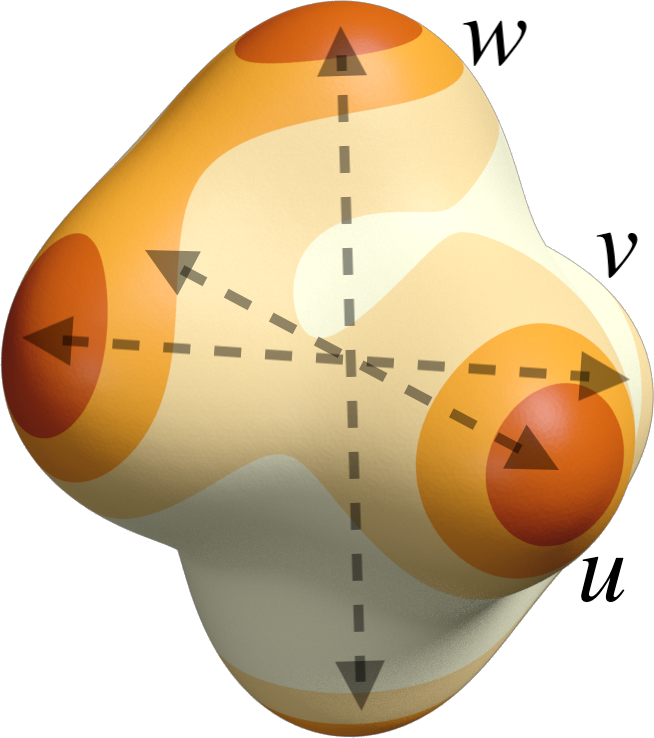
\includegraphics[width=0.8\linewidth]{img_spm_ff/sperical_3dir4_rot.png}
    \end{minipage}
    \begin{minipage}[c]{0.79\textwidth}
        %\centering
        %\includegraphics[width=0.33\linewidth]{sperical_3dir4.png}
        %$$P_\mathcal{U}(s) = const \cdot Y_{0, 0} + \sum_{m = -4}^4{{\color{green}c_{4, m}(\mathcal{U})}Y_{4,m}(s)}$$ 
        $$P_\mathcal{U}(s) = const \cdot Y_{0, 0} + \sum_{\ell \in \{2, 4\}} \sum_{m = -\ell}^\ell{{\color{green}c_{\ell, m}(\mathcal{U})}Y_{\ell,m}(s)}$$ 
    \end{minipage}
    
    \vspace*{.5\baselineskip}
    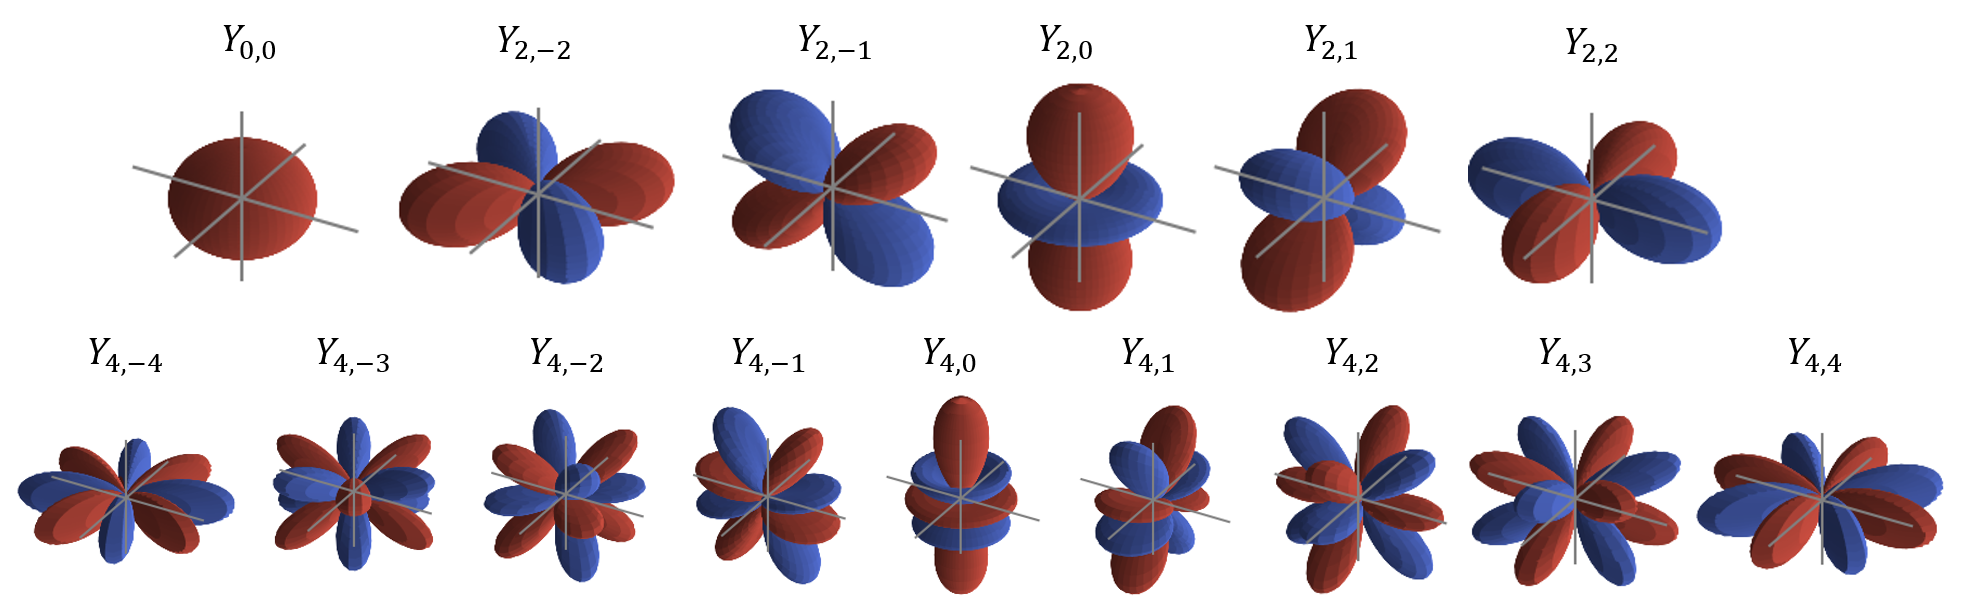
\includegraphics[width=\linewidth]{img_spm_ff/all_sph_harm.PNG} 
    \end{overprint}
\end{frame} 

\begin{frame}{Optimisation d'un champ de repère non-orthogonal 3D}
    \centering
    \footnotesize
     De la décomposition dans la base des Harmoniques, nous définissons:
    $$ dist(\mathcal{U}_i, \mathcal{U}_j) = \int (P_{\mathcal{U}_i} - P_{\mathcal{U}_j})^2 = \sum_{\ell, m} \left({\color{green}c_{\ell,m}(\mathcal{U}_i)} - {\color{green}c_{\ell,m}(\mathcal{U}_j)} \right)^2$$
    Pour calculer un champ de repère non-orthogonal 3D lisse, nous minimisons avec LBFGS l'énergie suivante :
    %To compute smoothed frame field, we minimize with LBFGS 
    $$ E_{tot} = \sum_{Voisins(i, j)} dist(\mathcal{U}_i, \mathcal{U}_j)$$
    %\vspace*{.5\baselineskip}
    %As in 2D, $\forall m,\ \ c_{2,m} \mapsto \lambda c_{2,m}$ modifies the orthogonality of the field. 
    Contrôle de l'orthogonalité: $\ \ c_{2,m} \mapsto \lambda c_{2,m} \ \ \ \ \ (-2 \leq m \leq 2)$ %modifies the orthogonality of the field. 
    
    \begin{minipage}[b]{0.33\textwidth}
        \centering
        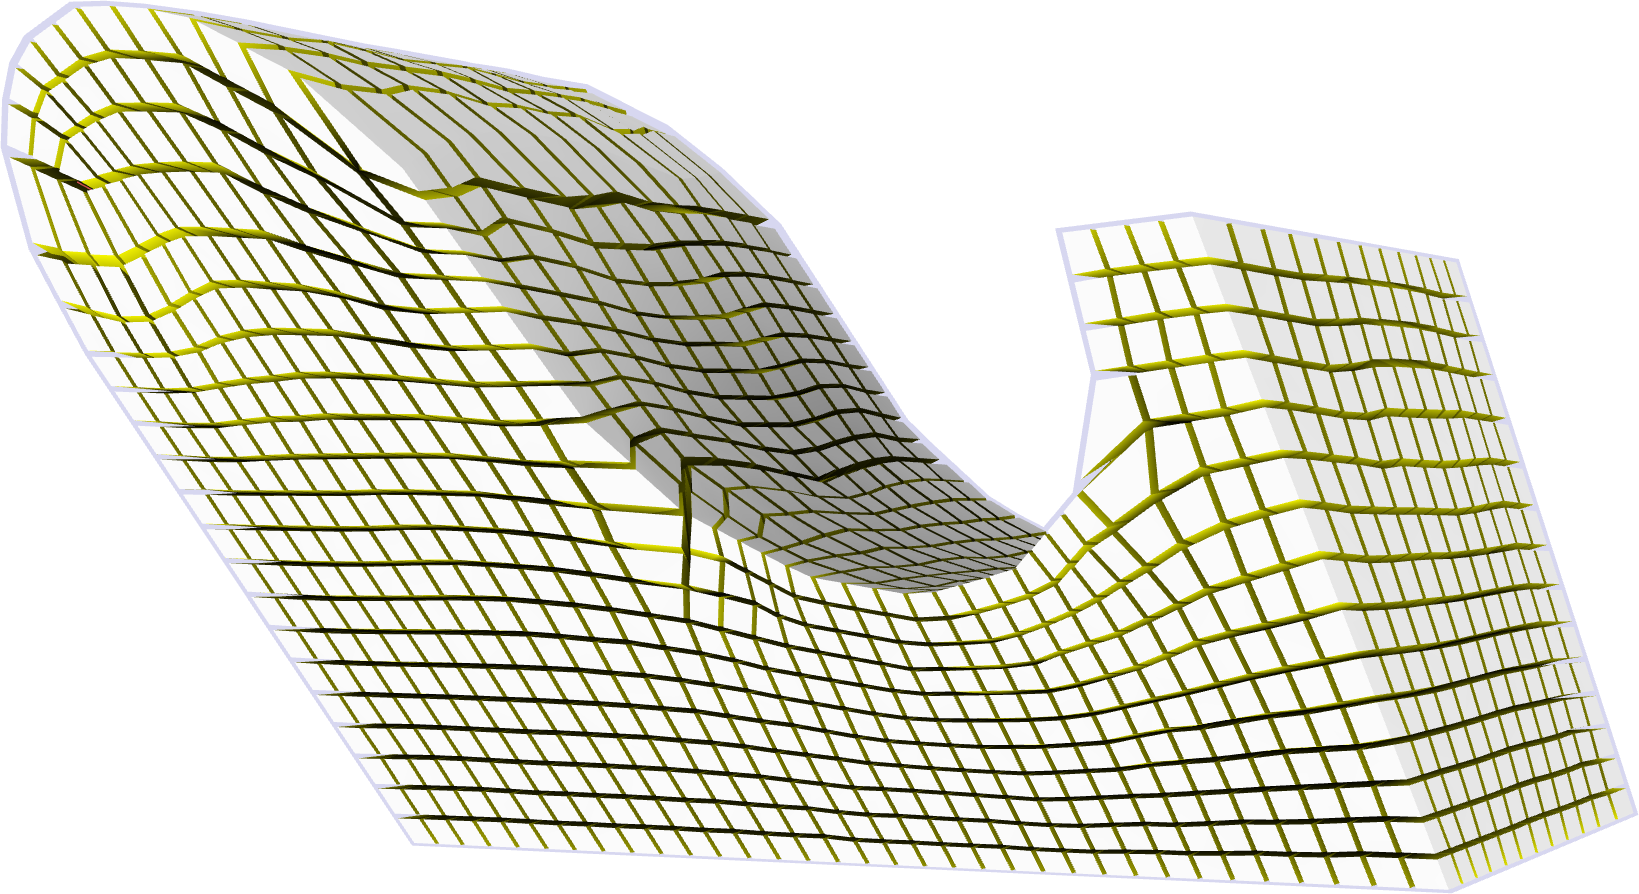
\includegraphics[width=\textwidth]{img_spm_ff/shear_0_7.png}
        $\lambda = 0.7$
    \end{minipage}
    \begin{minipage}[b]{0.28\textwidth}
        \centering
        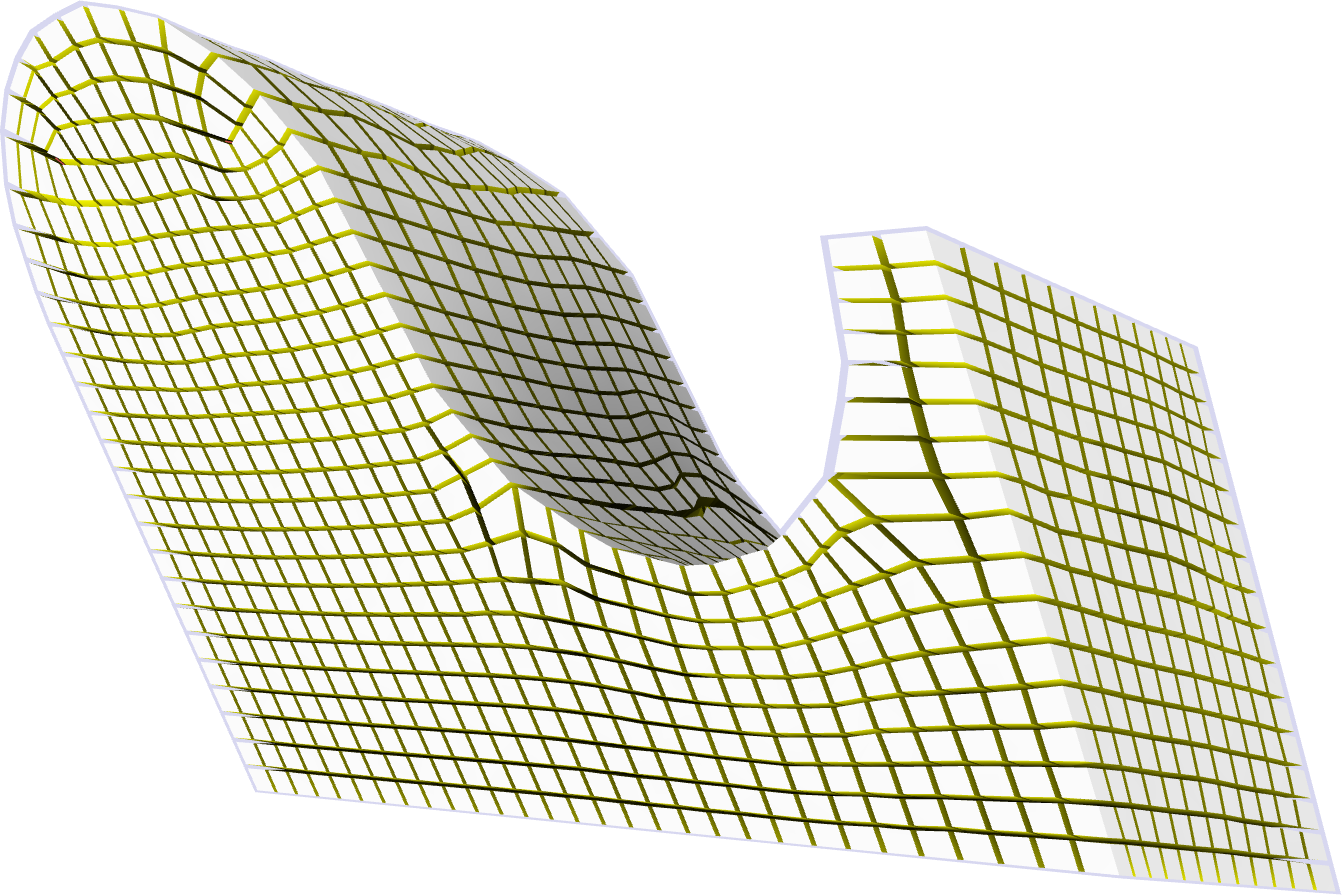
\includegraphics[width=\textwidth]{img_spm_ff/shear_1.png}
        $\lambda = 1$
    \end{minipage}
    
    \normalsize
\end{frame} 
